\documentclass[11pt, oneside]{article} 
\usepackage{geometry}
\geometry{letterpaper} 
\usepackage{graphicx}
	
\usepackage{amssymb}
\usepackage{amsmath}
\usepackage{parskip}
\usepackage{color}
\usepackage{hyperref}

\graphicspath{{/Users/telliott_admin/Dropbox/Tex/png/}}
% \begin{center} 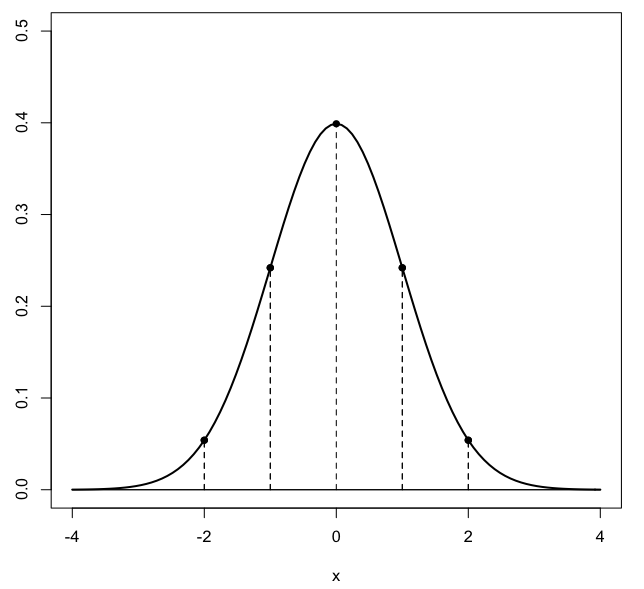
\includegraphics [scale=0.4] {gauss3.png} \end{center}

%break
\title{Generating functions}
\date{}

\begin{document}
\maketitle
\Large
\subsection*{generating functions}

$f(x)$ is a generating function for the sequence $a0$, $a1$, $a2$, $\dots$ if
\[ f(x) = \sum_{i = 0}^{\infty} a_i x^i \]
A generating function can sometimes be analyzed to prove something more (like a formula for the coefficients), but at the very least, it gives a way to generate them.

\subsection*{example}

The expected value for a function $f(x)$ of a continuous random variable is defined to be
\[ \int f(x) \ p(x) \ dx \]
For the exponential distribution $p(x) = \lambda e^{-\lambda x}$ we obtained
\[ E[x] = \int_0^{\infty} x \  \lambda e^{-\lambda x} \ dx \]
\[ E[x] = \frac{1}{\lambda} \]
using integration by parts (IBP).

(A note on nomenclature:  normally we would use $t$ as the variable when talking about the exponential distribution, since it's used for problems involving events happening in time.  But we're going to use $t$ for something else near the end, so just stick with $x$ here).

By two applications of IBP we obtained
\[ E[x^2] = \int_0^{\infty} x^2 \  \lambda e^{-\lambda x} \ dx \]
\[ E[x^2] = \frac{2}{\lambda^2} \]
Using these results we calculated the variance as
\[ \text{Var }(x) = E [(x - \mu)^2 ] \]
\[ = E[x^2] - (E[x])^2 \]
\[ = E[x^2] - \mu^2 \]
\[ = \frac{1}{\lambda^2} \]

\subsection*{generating function for exponential distribution}
A somewhat easier way is to do the same calculation is to use what is called the moment-generating function.  Here the variable $t$ is not for time but is instead a dummy variable.

\[ \phi(t) = \frac{\lambda}{\lambda - t}, \ \ t < \lambda \]
where the expected value of $x$ is the first derivative of $\phi(t)$ with respect to $t$, evaluated at $t=0$:
\[ E[x] = \frac{d}{dt} \ \phi(t) = \lambda \ \frac{1}{(\lambda - t)^2} \ \bigg |_{t=0} = \frac{1}{\lambda} \]
Similarly
\[ E[x^2] = \frac{d^2}{dt^2} \ \phi(t) = 2 \lambda \ \frac{1}{(\lambda - t)^3} \ \bigg |_{t=0}  = \frac{2}{\lambda^2}  \]
and so on.
This is certainly easier.  We obtain the third and fourth moments by the :same method
\[ E[x^3] = \frac{d^3}{dt^3} \ \phi(t) = 6 \lambda \ \frac{1}{(\lambda - t)^4} \ \bigg |_{t=0}  = \frac{6}{\lambda^3}  \]

Of course, the question is then:  where does $\phi(t)$ come from?  
\subsection*{derivation}
According to

\url{https://www.statlect.com/fundamentals-of-probability/moment-generating-function}

With some restrictions (notably $t < \lambda$):
\[ E[ e^{tX} ]  =  \int_{-\infty}^{\infty}  e^{tx} \ p(x) \ dx \]
Recall that for the exponential distribution, the pdf is
\[ p(x) = \lambda e^{-\lambda x} \]
so we have
\[ \int_{-\infty}^{\infty}  e^{tx} \lambda e^{-\lambda x} \ dx \]
The probability is defined to be $p(x) = 0$ for $x < 0$ so the bounds change to
\[ \int_{0}^{\infty}  e^{tx} \lambda e^{-\lambda x} \ dx \]
\[ = \lambda \int_{0}^{\infty}  e^{(t - \lambda)x} \ dx \]
which we note is only finite for $t < \lambda$.  The integral is pretty easy but the bounds make it improper:
\[ = \frac{\lambda}{t - \lambda} \ e^{(t - \lambda)x} \ \bigg |_{0}^{\infty} \]
Now, since $t < \lambda$ and so $t- \lambda < 0$), this is a negative exponential $e^{-kx}$.

Therefore, the upper bound is just zero.  The exponential in the lower bound becomes $1$ and subtraction of the rest gives:
\[ \frac{\lambda}{\lambda - t}  \]
So that is the immediate derivation, which doesn't say much about \emph{why} it works, of course.

More generally, we can write
\[  E[ e^{tX} ]  = \int  e^{tx} \ p(x) \ dx \]
We expand the exponential as a power series:
\[ = \int  (1 + tx + \frac{t^2x^2}{2} + \dots) \ p(x) \ dx \]
\[ = \int \ p(x) \ dx + \int tx \ p(x) \ dx + \int t^2x^2 \ p(x) \ dx  + \dots \]
\[ = 1 + t E(x) + t^2 E(x^2) + \dots \]
So we can see why, to get the kth moment, we take the kth derivative with respect to $t$ and then evaluate with $t=0$ to knock out all the higher terms.

And \emph{that's} why it works.

\subsection*{Another approach}
A moderately advanced (but simplifying) technique that can be used to solve this same problem is called differentiating under the integral sign.  

Before we go through that, just review the following improper integral
\[ \int_0^{\infty} e^{-cx} \ dx \]
for some constant $c$.  We solve the integral with a real positive number $b$ as the upper bound
\[ \int_0^{b} e^{-cx} \ dx = -\frac{1}{t} e^{-cx} \bigg |_0^b = -\frac{1}{c} \ [ \ e^{-cb} - 1 \ ] \ \]
In the limit as $b \rightarrow \infty$, the negative exponential first term goes to zero, so we have simply
\[ \int_0^{\infty} e^{-cx} \ dx = \frac{1}{c} \]

Liebnitz's rule says that you can differentiate on either side of the integral sign
\[ \frac{d}{dt} \ \int_0^{\infty} e^{-tx} \ dx = \int_0^{\infty} \frac{\partial}{\partial t} \  e^{-tx} \ dx \]

Use the result from above that this integral is just $1/t$ so the left-hand side is:
\[ \frac{d}{dt} \ \frac{1}{t} = - \frac{1}{t^2} = - t^{-2} \]
Differentiate \emph{with respect to} $t$ on the right-hand side:
\[ - t^{-2} = \int_0^{\infty} -x \  e^{-tx} \ dx \]
Rearranging:
\[ \int_0^{\infty} x e^{-tx} \ dx = t^{-2} \]

This can be continued indefinitely:
\[ \int_0^{\infty} x^2 e^{-tx} \ dx = 2 t^{-3} \]
Here we have simply repeated the differentiation with respect to $t$ on both sides, while canceling the minus signs.

There is more in the write-up on the technique.

Solving our problem
\[ E[x] = \int_0^{\infty} x \  \lambda e^{-\lambda x} \ dx \]
we get $\lambda$ times what we have above, namely
\[ \lambda \ \int_0^{\infty} x e^{-\lambda x} \ dx = \lambda \ \lambda^{-2} \]
Thus, cancelling one factor of $\lambda$ on top and bottom we obtain:
\[ E[x] = \frac{1}{\lambda} \]

Similarly

\[ E[x^2] = \lambda \ \int_0^{\infty} x^2 e^{-\lambda x} \ dx \]
\[ = \lambda \ 2 \lambda ^{-3} = \frac{2}{\lambda^2} \]



\end{document}  